\chapter{物体内部に配置したBLEビーコンの電波強度を用いた状態推定}
\thispagestyle{myheadings}

\begin{figure}[tbh]
    \centering
    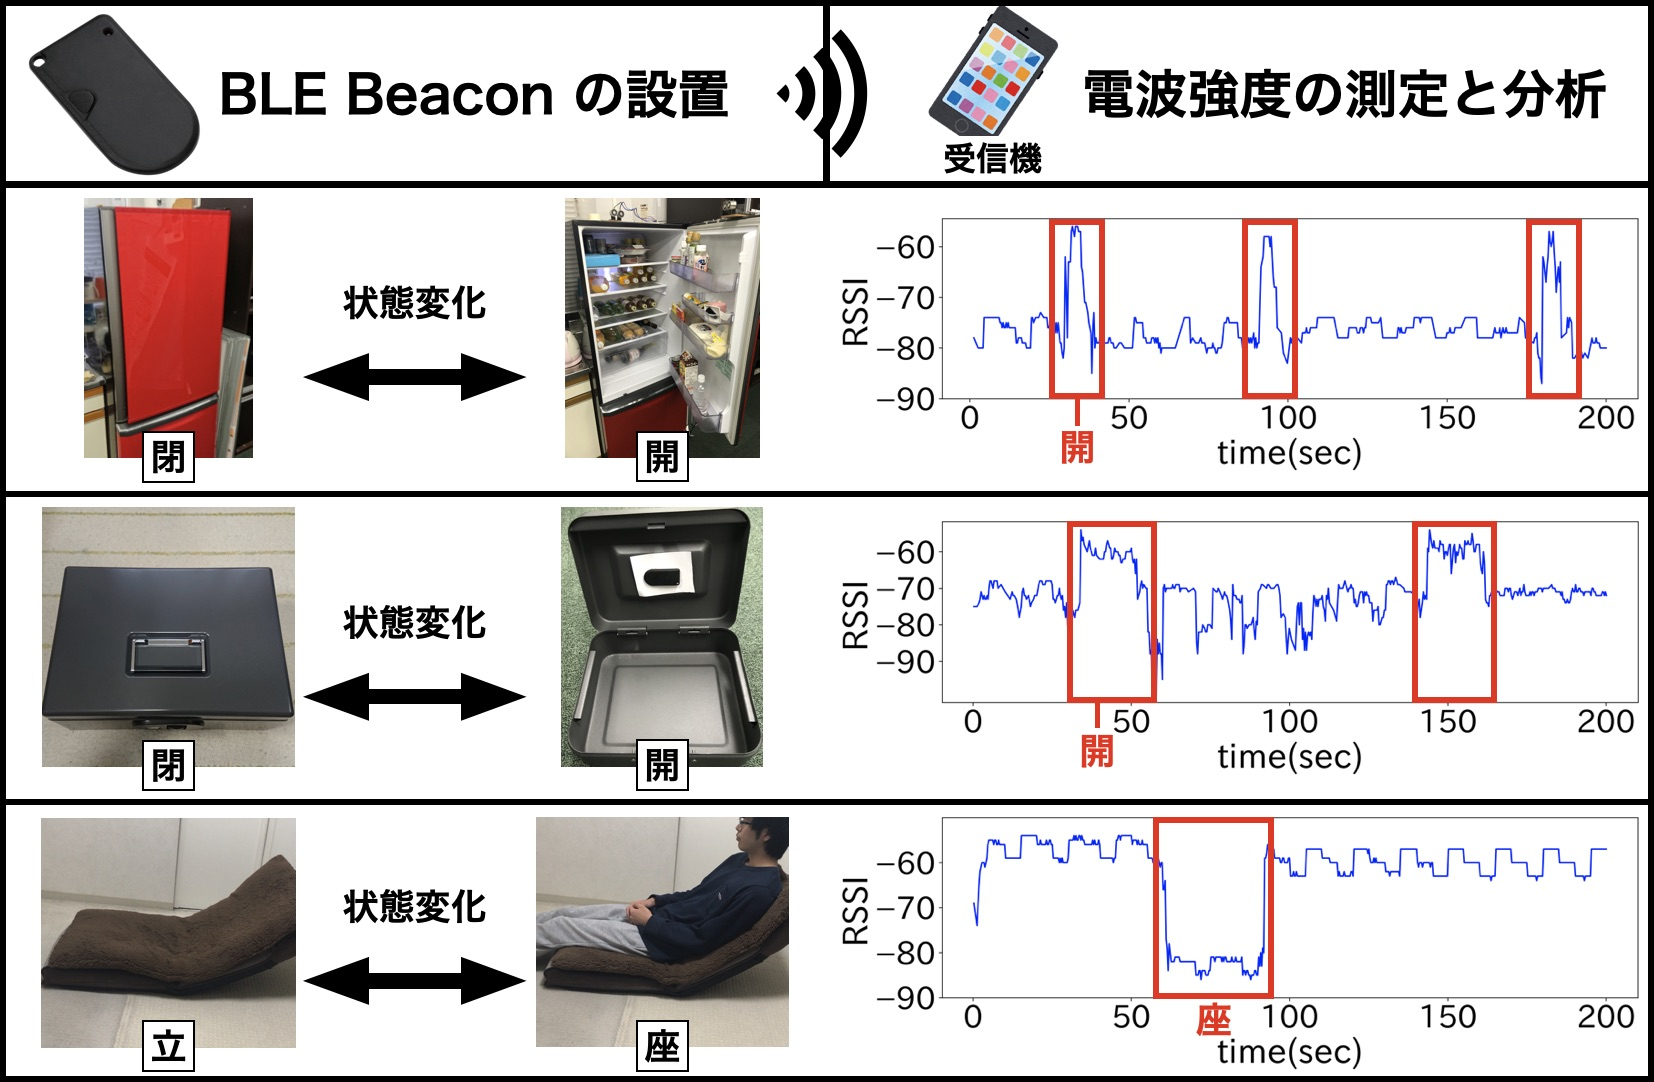
\includegraphics[width=14cm]{images/chapter3/abst.jpg}
    \caption{提案手法概要}
    \label{abst-chap3}
\end{figure}

本研究では屋内にあるモノの内部に直接BLEビーコンを設置し,その状態変化による電波強度の変化からモノの状態推定を行う.
提案手法の概要図を図\ref{abst-chap3}に示す.
本稿では材質や使用方法によって受信電波強度に大きな変化が現れるモノを対象として,状態推定を行う.
具体的には,冷蔵庫と金庫,座椅子である.
冷蔵庫(図\ref{freezer})では扉の棚部分,金庫(図\ref{safe})では開閉する蓋の部分,座椅子(図\ref{chair})では人が座る座面の部分や背もたれの部分へ図\ref{beacon}のBLEビーコンを設置する.
冷蔵庫や金庫では金属による電波の減衰が起き,座椅子では人体によって電波の減衰が起こる.
これにより,扉の開閉や人の着座などのモノの状態変化からBLEビーコンの遮蔽状態が変化するため,外側に設置した受信機での受信電波強度が変化する.
この変化する電波強度をもとにモノの状態変化の推定を行う.



\begin{figure}[H]
    \centering
    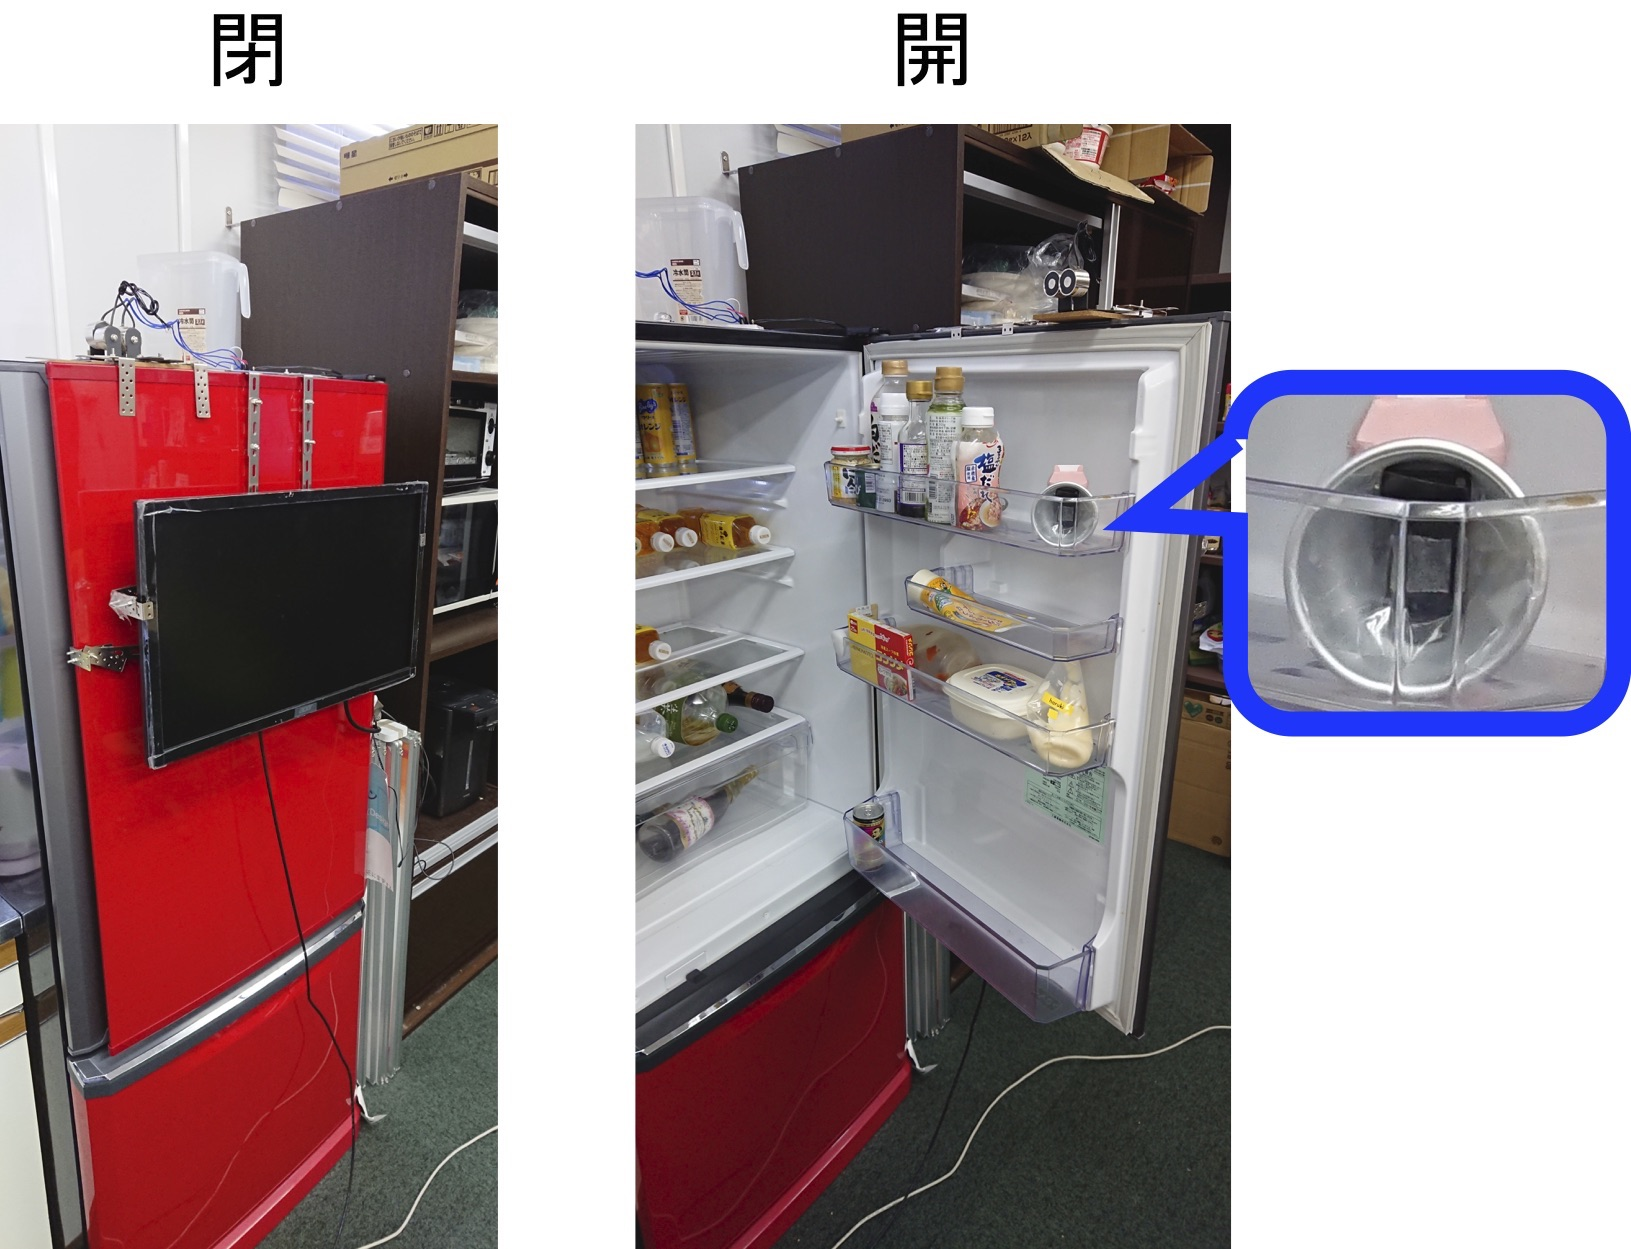
\includegraphics[width=10cm]{images/chapter3/regisW2.jpg}
    \caption{冷蔵庫の状態と設置したBLEビーコン}
    \label{freezer}
\end{figure}


\begin{figure}[H]
    \centering
    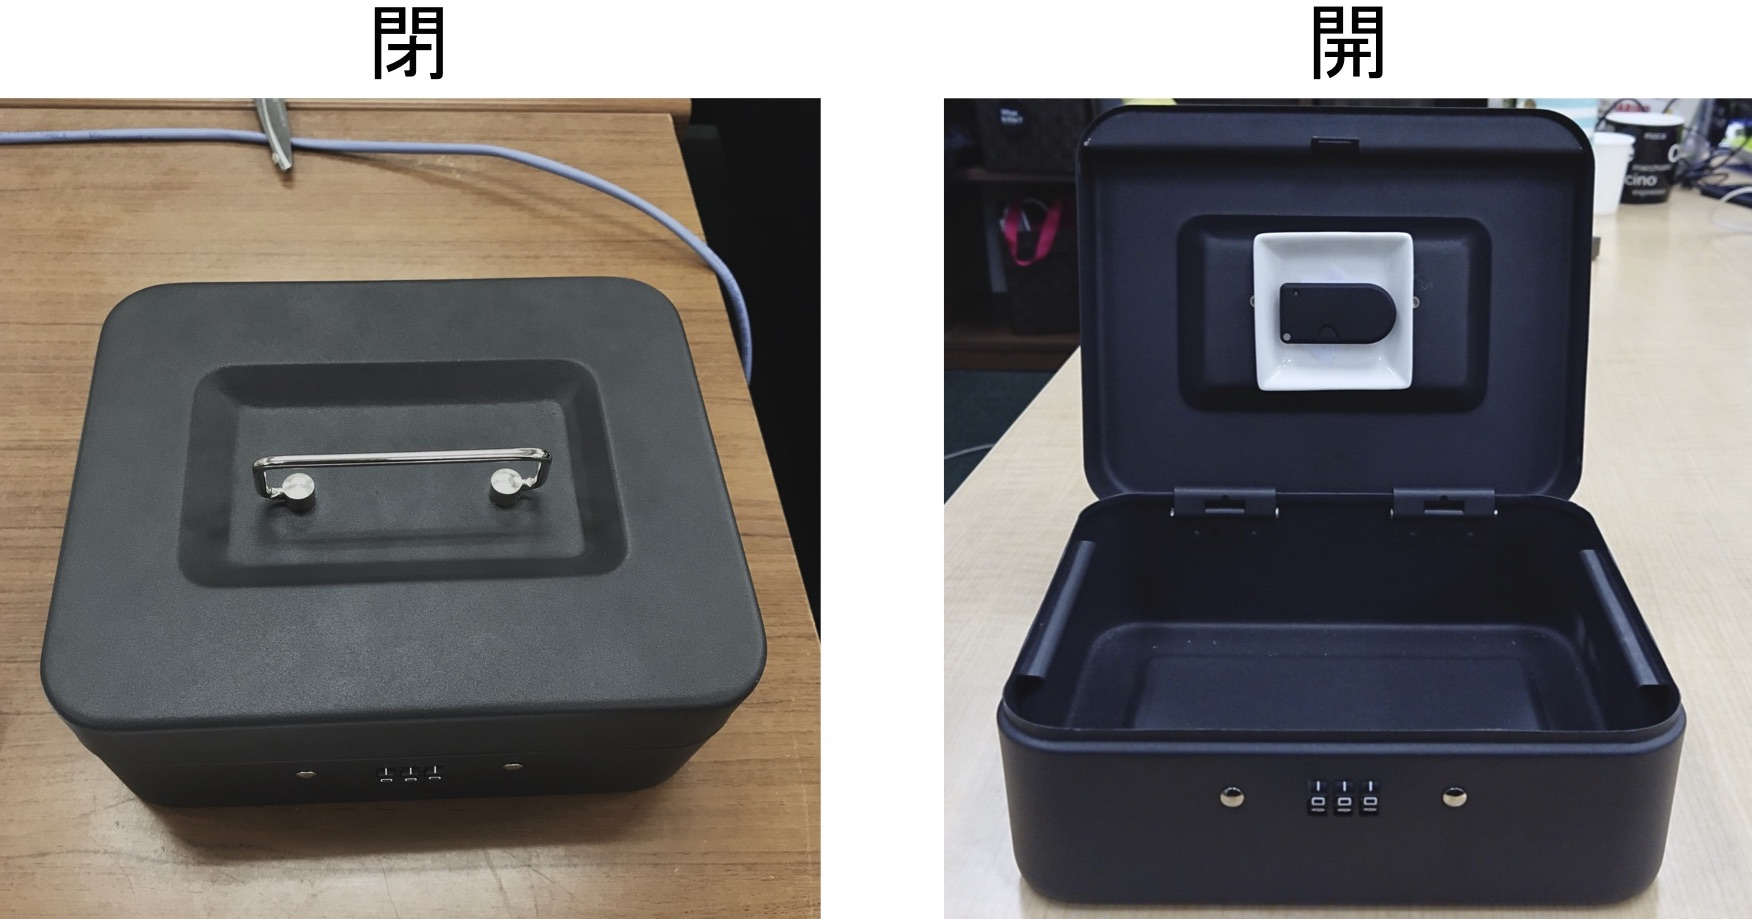
\includegraphics[width=10cm]{images/chapter3/kinkoW.jpg}
    \caption{金庫の状態と設置したBLEビーコン}
    \label{safe}
\end{figure}


\begin{figure}[H]
    \centering
    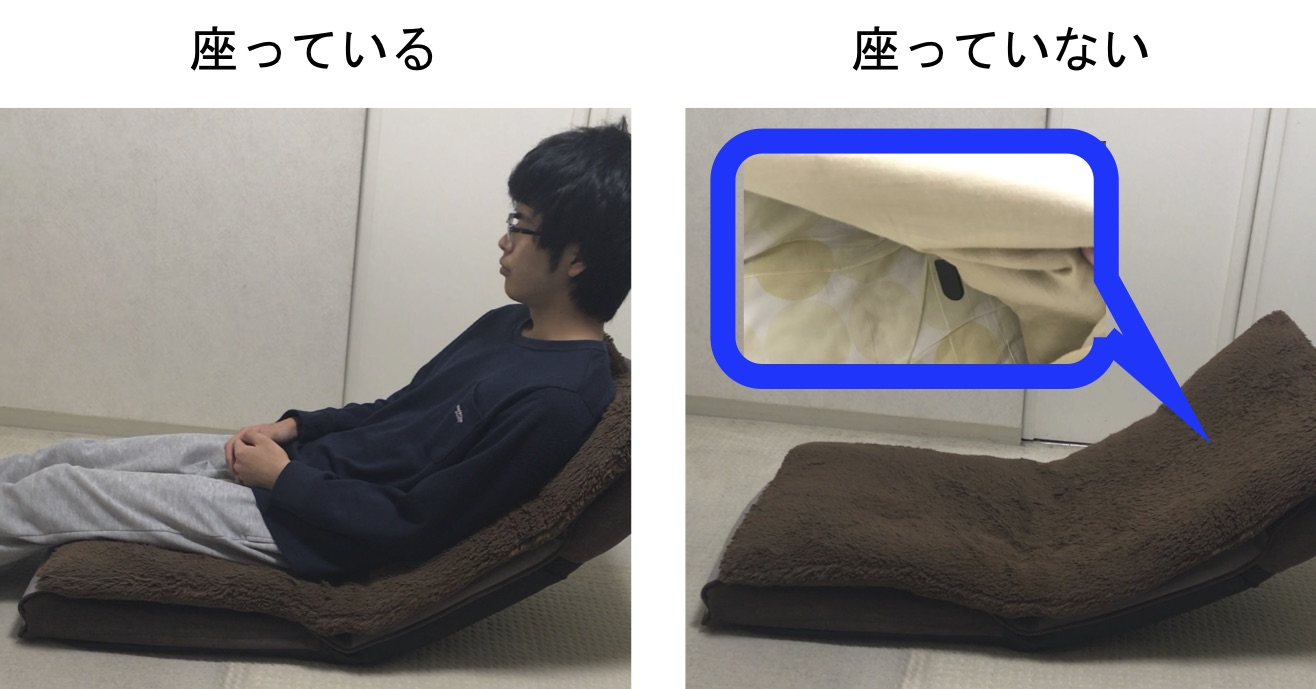
\includegraphics[width=10cm]{images/chapter3/zaisuW.jpg}
    \caption{座椅子の状態と設置したBLEビーコン}
    \label{chair}
\end{figure}


\begin{figure}[tbh]
    \centering
    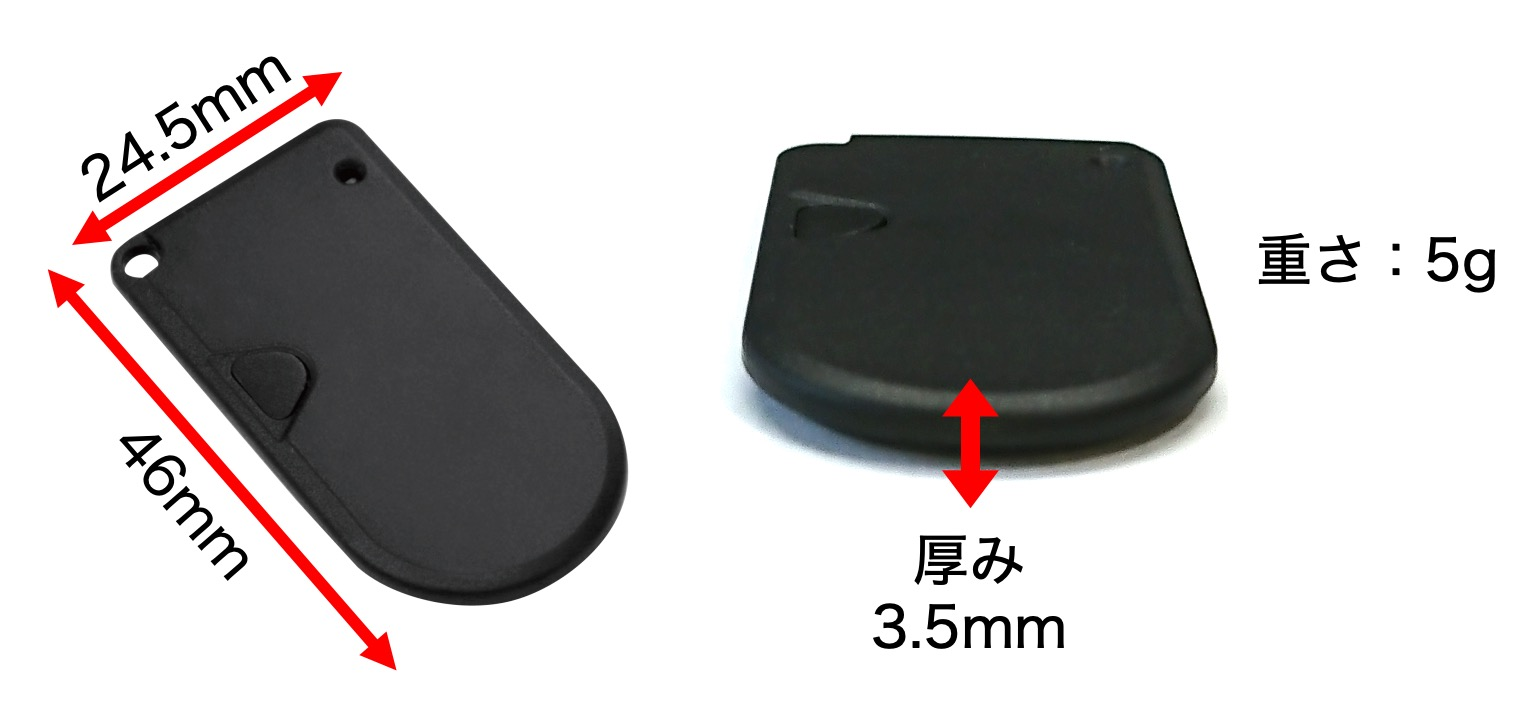
\includegraphics[width=10cm]{images/chapter3/BLE_beacon_info.jpg}
    \caption{BLEビーコン}
    \label{beacon}
\end{figure}


%ーーーーーーーーーーーーーーーーーーーーーーーーーーーーーーーーーーーーーーーーーーーーーーーーー
%ーーーーーーーーーーーーーーーーーーーーーーーーーーーーーーーーーーーーーーーーーーーーーーーーー


\section{BLEビーコンの取り付け位置の検討と設定}
本研究では,モノの状態が変化した際のBLEビーコンの電波強度変化をもとに状態推定を行う.
そのため,BLEビーコンはその変化が一番大きくなる位置に設置する必要がある.
例えば,箱型で蓋の開閉を行う金庫のようなものであれば,BLEビーコンを箱内部の底に設置する場合と,蓋の裏に設置する場合が考えられる(図\ref{adapter}).
また,モノの材質によっては電波を通しやすく,状態変化しても電波強度に大きな変化が現れないモノもある.
そこで,図\ref{adapter}の右側に示すようにBLEビーコンに対して指向性アダプタを取り付ける.
この指向性アダプタとは,図\ref{adapter_only}に示す金属や陶器でできたパラボラアンテナのような形状の物を指す.
取り付けた際の効果として,電波が拡散せず収束して一方向のみへ飛ぶようになり,状態変化によって電波強度に大きな変化が現れるようになる.


\begin{figure}[H]
    \centering
    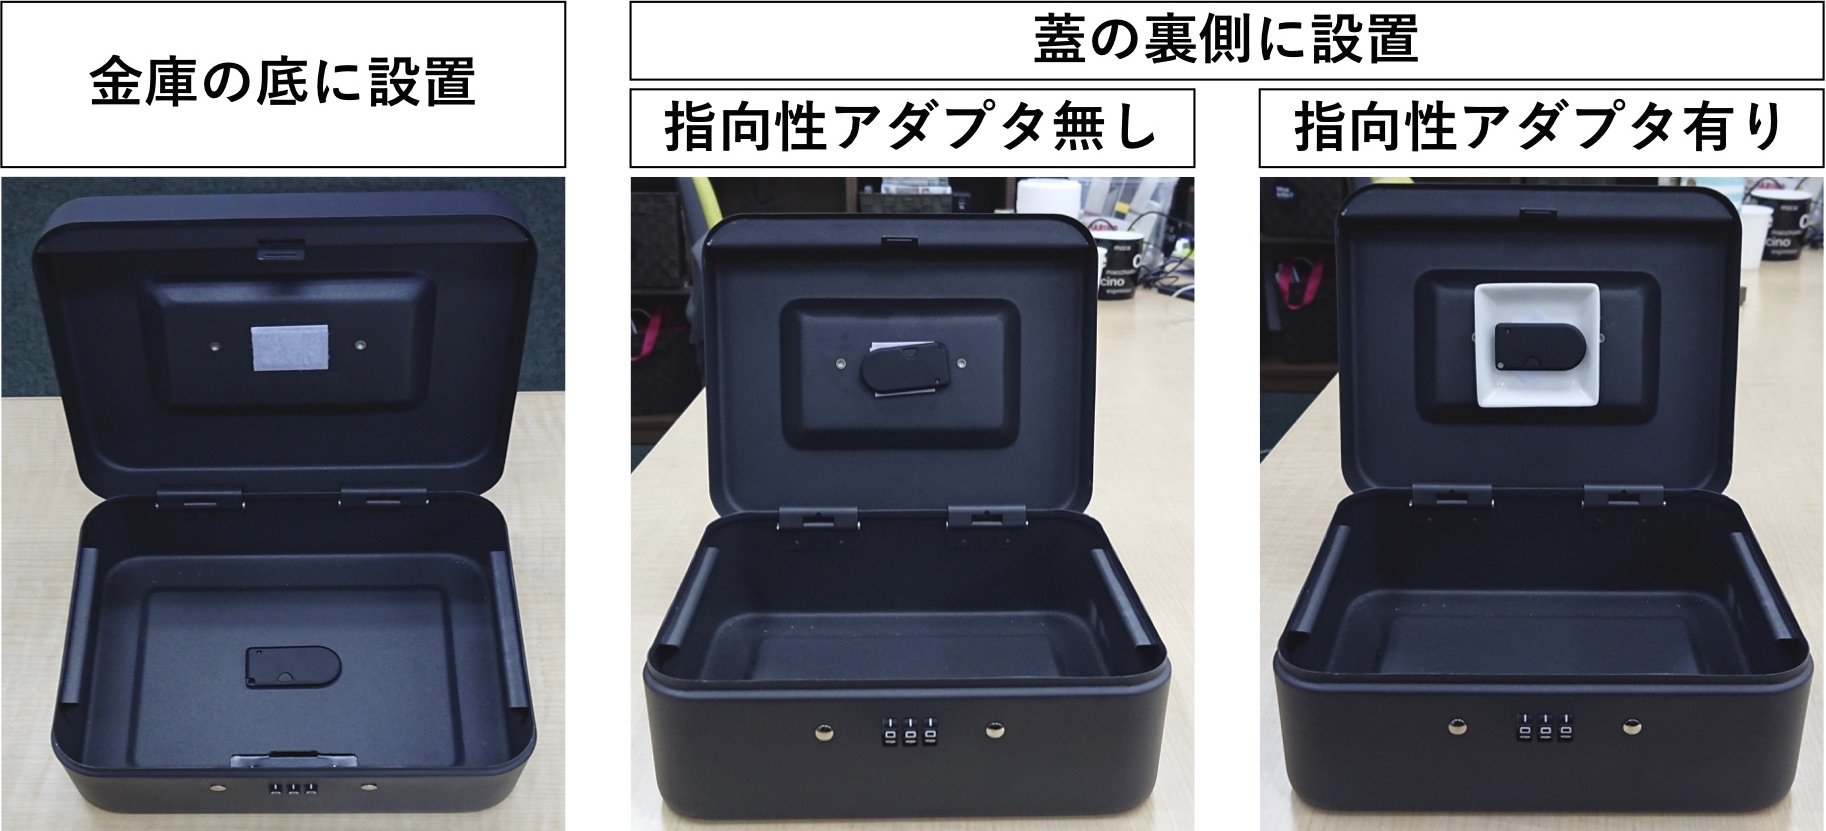
\includegraphics[width=12cm]{images/chapter3/adapta_compare.jpg}
    \caption{BLEビーコンの設置場所と指向性アダプタ}
    \label{adapter}
\end{figure}


\begin{figure}[H]
    \centering
    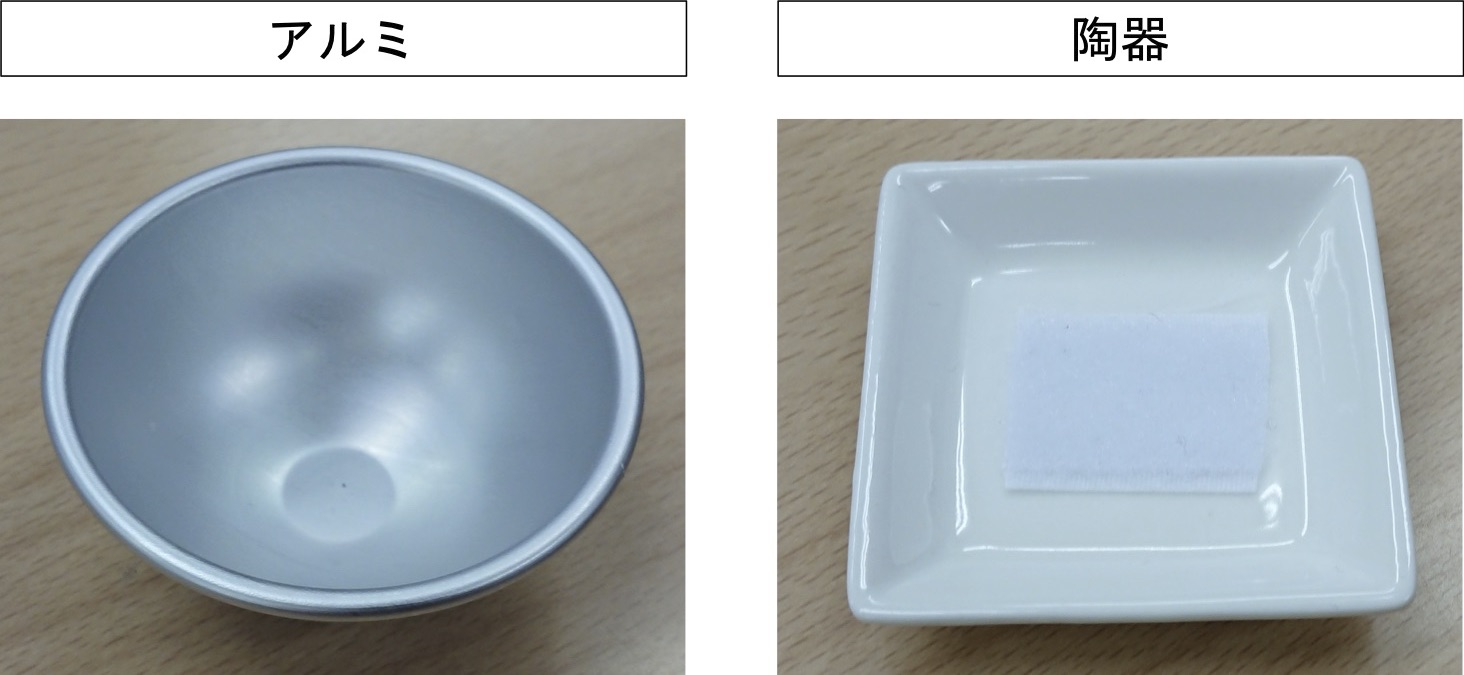
\includegraphics[width=12cm]{images/chapter3/adapta.jpg}
    \caption{本研究で使用した指向性アダプタ}
    \label{adapter_only}
\end{figure}


図\ref{transform-data}にそれぞれの取り付け方による金庫開閉時の電波強度の波形を示す.
この図にはそれぞれ開いている状態と閉じている状態の正解ラベルをつけている.
BLEビーコンを金庫内部の底につけた場合にはあまり大きな変化は見られず,蓋の裏側にBLEビーコンを設置した場合では大きな変化が見られる.
さらに,指向性アダプタをつけた場合には,よりくっきりと電波強度に差が現れる.
このように,状態推定対象物に合わせてBLEビーコンの取り付け方を工夫し,状態推定の高精度化を図る.

本研究では受信機としてスマートフォンを使用するため,専用のAndroidアプリケーションを作成し,電波強度の情報を収集する.
その際,BLEビーコンを識別するためのUUID,major,minorをBLEビーコンを設置する対象と紐付けし,どのBLEビーコンの値がどの対象物のモノなのか把握できるようにしている.
また,小さな変化も検知できるようにBLEビーコンの電波送信設定は,送信強度は0dBm,送信間隔は100msと設定している.

\begin{figure}[H]
    \centering
    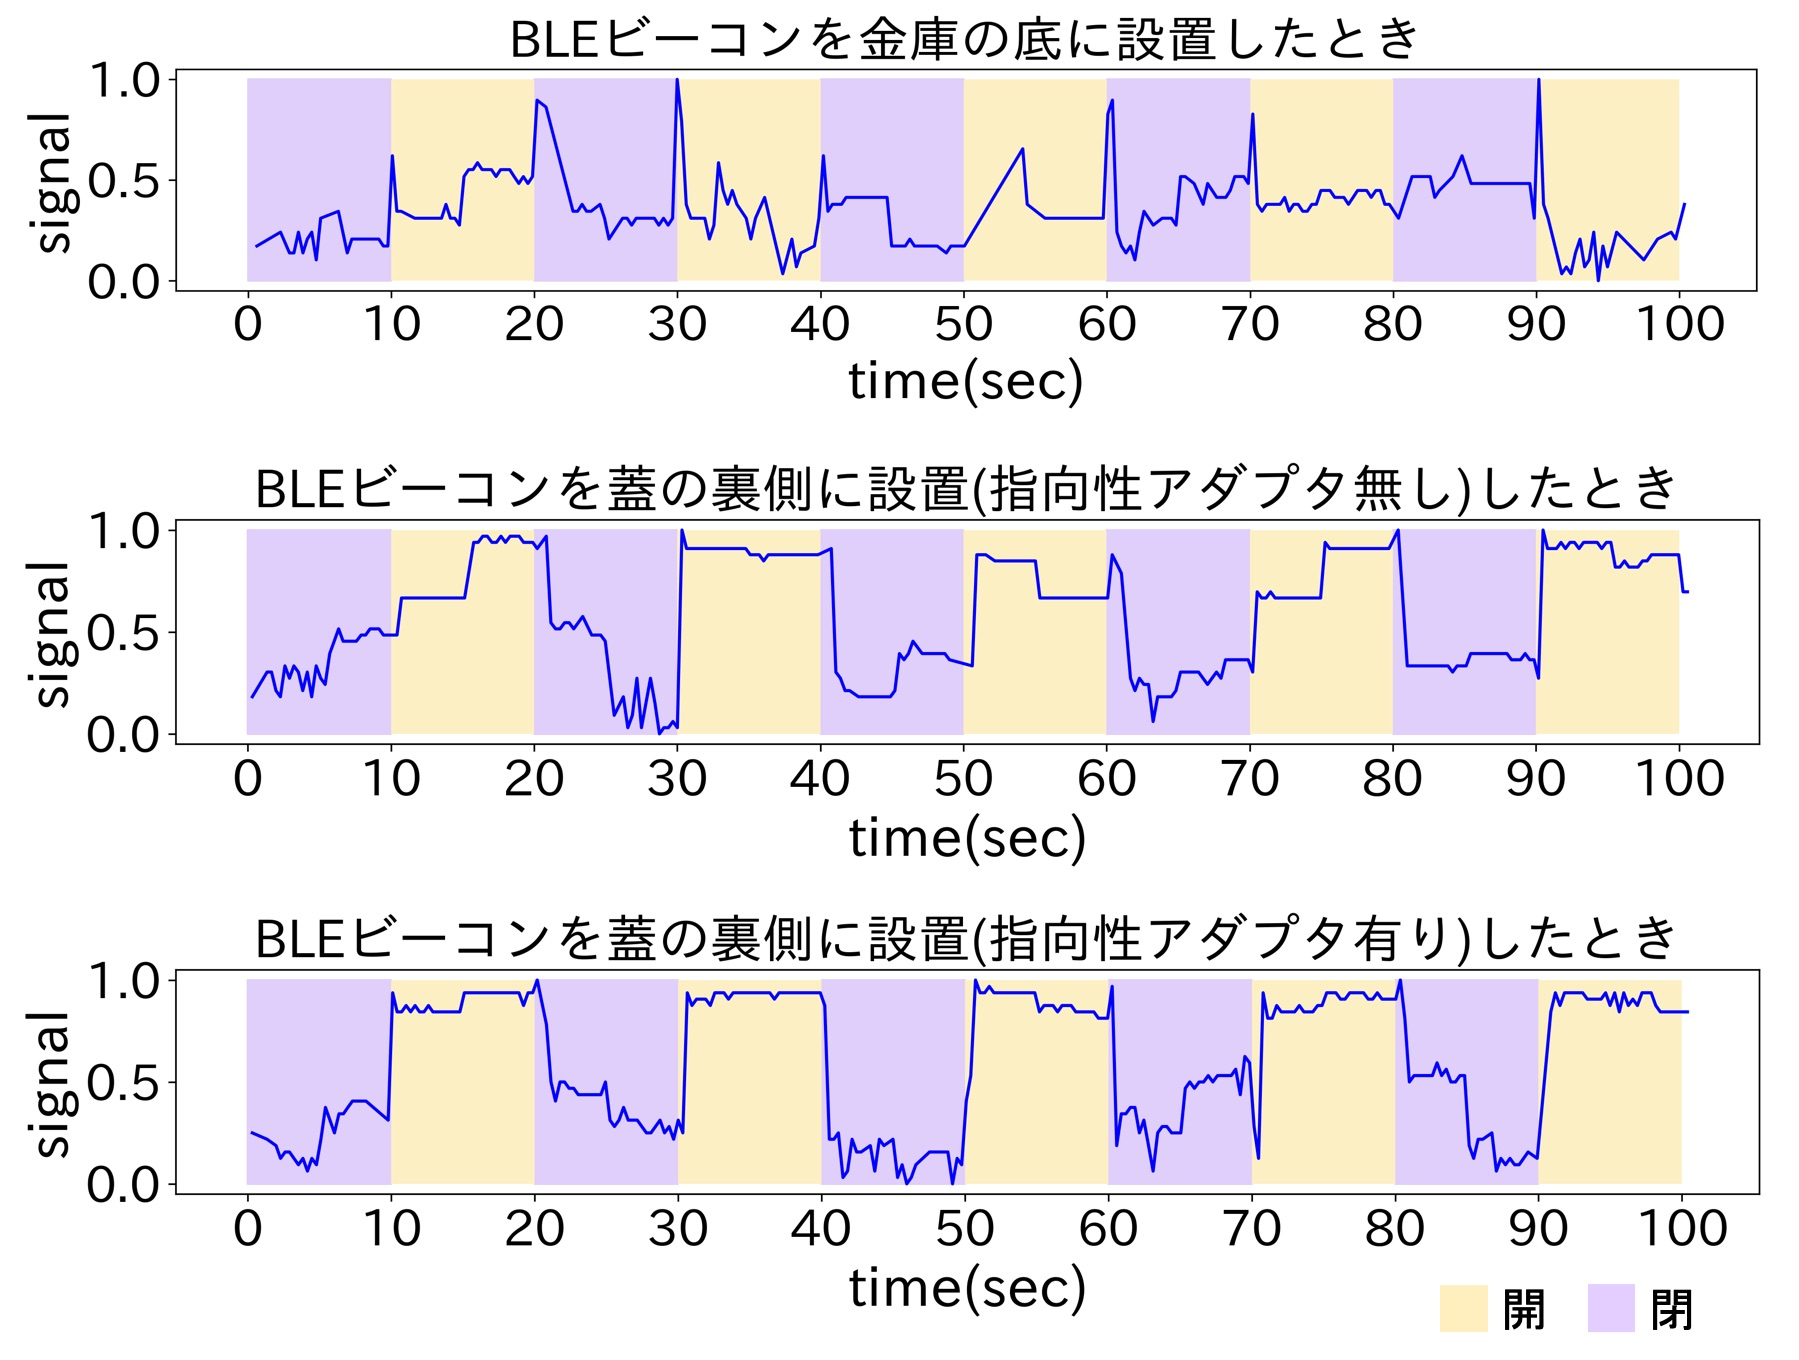
\includegraphics[width=14cm]{images/chapter3/in-out.jpg}
    \caption{BLEビーコン取り付け位置ごとの電波強度変化}
    \label{transform-data}
\end{figure}


%ーーーーーーーーーーーーーーーーーーーーーーーーーーーーーーーーーーーーーーーーーーーーーーーーー
%ーーーーーーーーーーーーーーーーーーーーーーーーーーーーーーーーーーーーーーーーーーーーーーーーー


\section{状態推定アルゴリズム}

\begin{figure}[tbh]
    \centering
    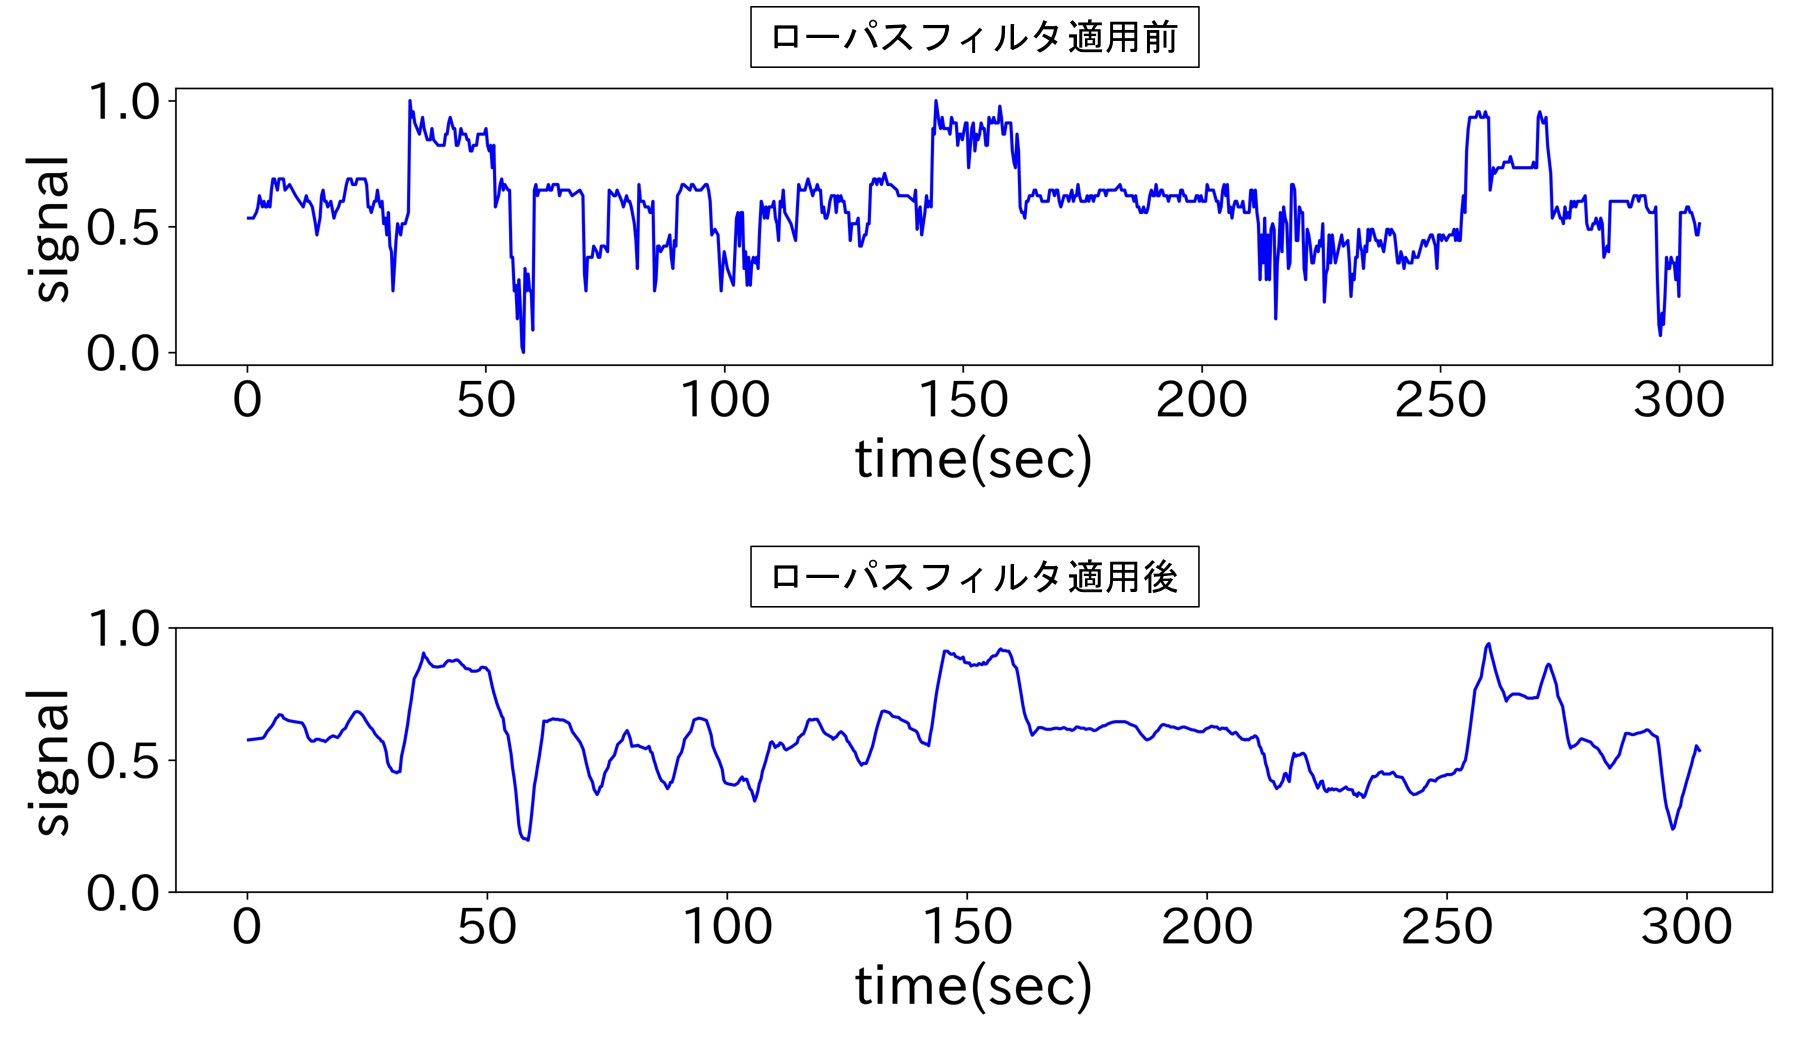
\includegraphics[width=14cm]{images/chapter3/lowpath_compare.jpg}
    \caption{ノイズ軽減処理前後の波形比較}
    \label{bank-opcl}
\end{figure}

本手法ではBLEビーコンから発せられる電波を300msの間隔で受信し,その受信電波強度の値から状態を推定する.
このとき,取得したデータをそのまま使用すると,ノイズによる影響を受けてしまい正確に推定を行えない.
そこで,取得したデータに対して複数の処理を適用し,ノイズの軽減を図る.
ノイズを軽減するための処理として,本手法ではローパスフィルタと正規化を使用する.
このとき,ローパスフィルタには10個のサンプル,つまり3秒分のデータを用いる.
図\ref{bank-opcl}に金庫の蓋を開閉した際の電波強度変化グラフと,ノイズ軽減処理の結果を示す.

% \subsection{安定センシング区間}
本手法では推定対象物の移動も考慮する.
しかし,物体が状態変化をせず移動した場合や人の往来,BLEビーコンの発する電波の揺らぎなどによって受信電波強度が安定しない場合がある.
% しかし,物体が状態変化をせず移動した場合,電波強度は徐々に変化するため閾値を用いた単純な推定では誤判定が起きてしまう.
そこで,梶ら\cite{sensing-area}が提案している安定センシング区間という概念を利用し,推定精度の高精度化を図る.
安定センシング区間とは,一定時間以上センシングが安定して行えている区間を指す.
本研究ではある値に着目した際に,その値が基準となる値の上限・下限閾値の範囲内であり,かつ一定時間以上経過している区間がそれにあたる.

図\ref{nomal-data}はBLEビーコンを遮蔽物のない環境で測定した電波強度のグラフであるが,ここからBLEビーコンの電波は電波強度が周期的に変化しているのがわかる.
このBLEビーコン特有の周期的な電波強度変化により安定センシング区間の判定が不安定になるため,上限・下限閾値は使用するBLEビーコンや推定対象物の特徴に合わせて設定を行う.
もし,閾値を超えた場合は,超える直前の受信電波強度の値に±Xした値を新しい閾値として設定する.
これにより推定対象物が移動しても状態推定が可能となる.

\begin{figure}[tbh]
    \centering
    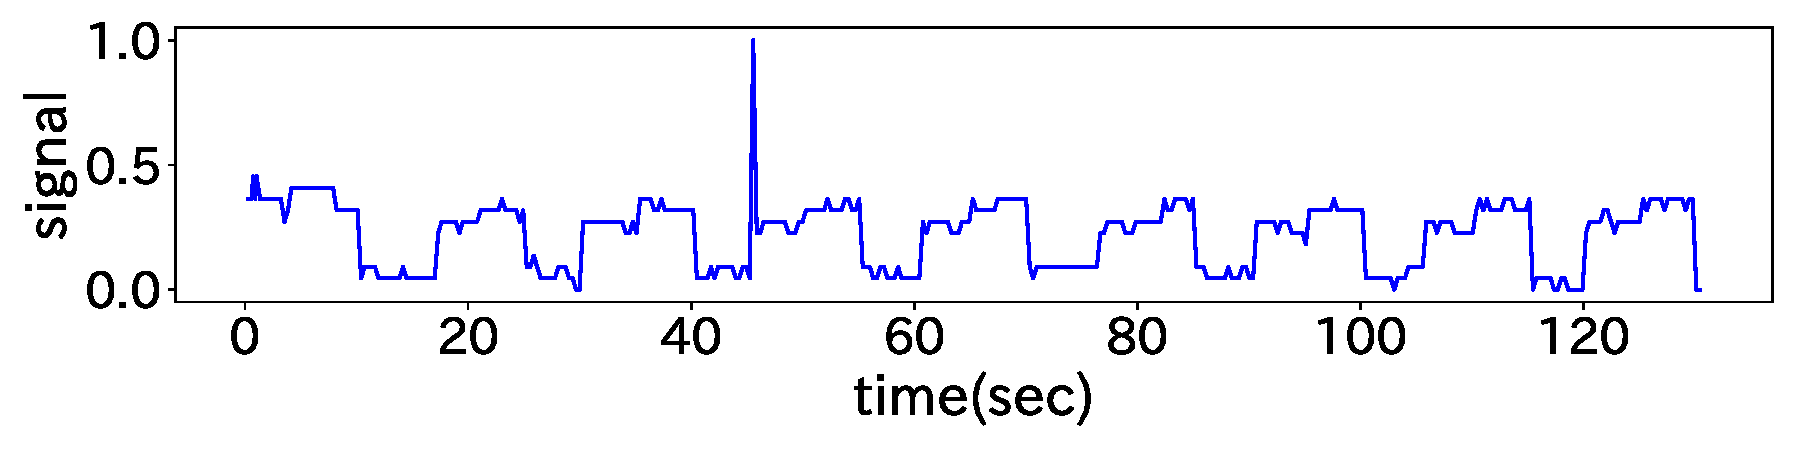
\includegraphics[width=14cm]{images/chapter3/bokoboko.pdf}
    \caption{BLEビーコンを遮蔽物のない状態で測定した電波強度グラフ}
    \label{nomal-data}
\end{figure}

% \subsection{状態変化の推定}
安定センシング区間の判定が終わったら,見つけた各区間がポジティブな状態か,ネガティブな状態か判定を行う.
ポジティブな状態とはBLEビーコンが外に出ていて電波の受信がしやすく、電波強度の値が大きい状態を指す.
具体的には金庫の開閉であれば開いてる状態である.
ネガティブな状態とはBLEビーコンが外に出ておらず電波の受信が難しく、電波強度の値が小さい状態を指す.
具体的には金庫の開閉であれば閉じてる状態である.
判定は,各安定センシング区間の受信電波強度の平均値が,全受信電波強度の中央値に0.1を足した値より大きいか小さいかで行う.


\section{エフェクト表示}



\subsection{実験端末の選定}

\begin{figure}[tbh]
    \centering
    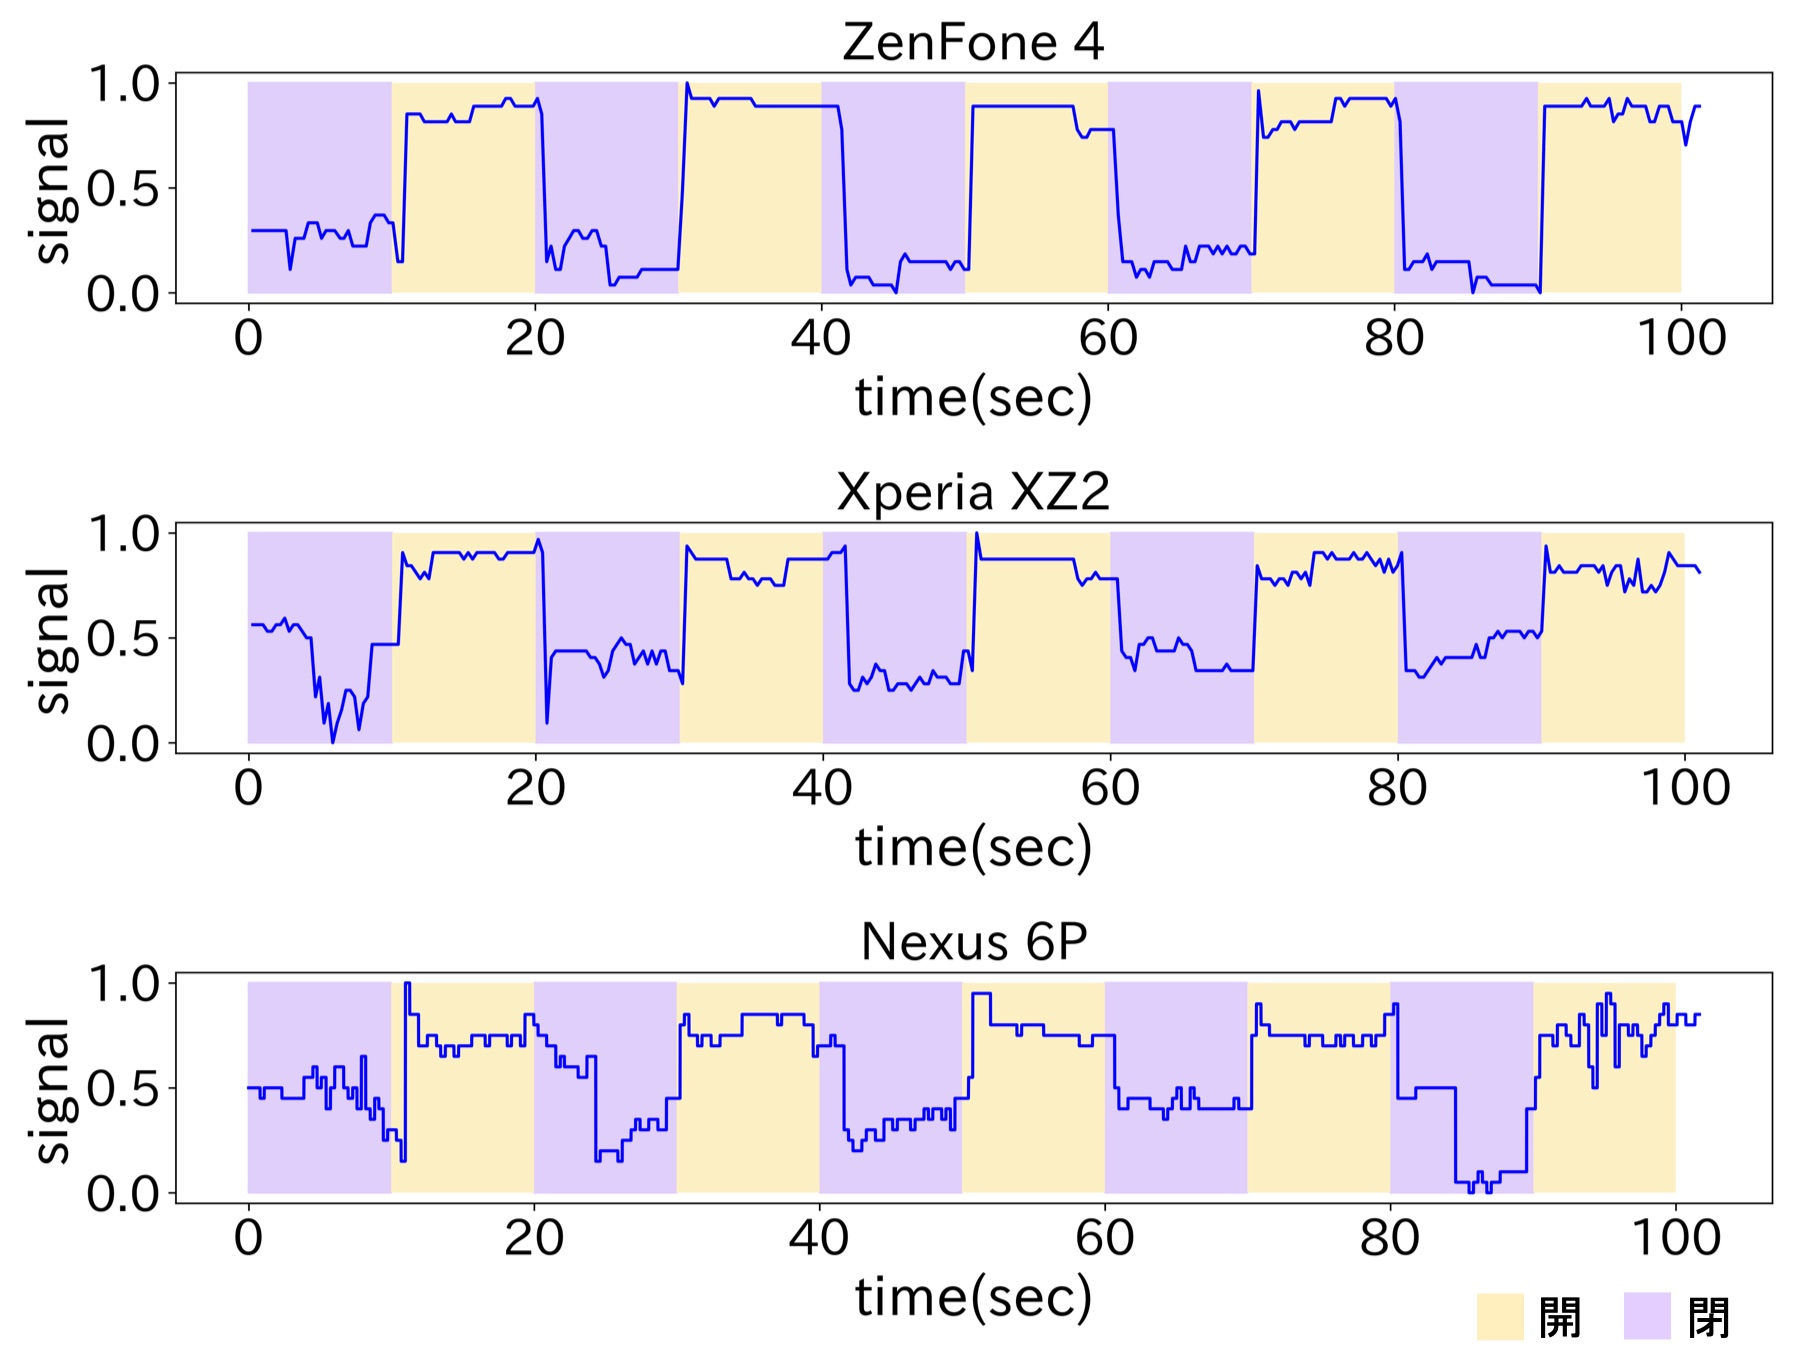
\includegraphics[width=14cm]{images/chapter3/mix.jpg}
    \caption{機種ごとの精度比較}
    \label{multi-data}
\end{figure}

Bluetoothのセンサ精度は端末ごとに異なるため,実験に用いる端末は変化を正しく捉えられる端末を使うのが望ましい.
そこでAndroid端末を3機種用意し,同一環境下で金庫の蓋の開閉を行い測定精度の比較を行った.
今回用意した端末はXperia XZ2,Nexus 6P,ZenFone 4である.
金庫開閉時の電波強度変化を各端末で収集し,その波形を比較した結果を図\ref{multi-data}に示す.
図の紫色の部分は蓋が閉まっている状態を黄色の部分は蓋が開いている状態を示している.
3機種の精度を比較した結果,Nexus 6Pでは全体的に小さなノイズが発生しているがZenFone 4とXperia XZ2ではそれが少ない.
また,Xperia XZ2とNexus 6Pは測定開始直後は測定値が安定せず正しく変化を捉えられていない.

本手法では電波強度の急激な変化と安定センシング区間の判定が重要となるため,測定ノイズが少なく電波を正確に捉えられる必要がある.
そこで,この3機種のうち一番ノイズが少なかったZenFone 4を実験で用いる受信機として採用した.
また,本研究では金庫などの移動を伴う比較的小さなモノにもBLEビーコンを取り付けるため,使用するBLEビーコンはできるだけ小さい方が望ましい.
そのためBLEビーコンは軽量・小型という理由からフォーカスシステムズ社のFCS1301(図\ref{beacon})を使用した.


\subsection{冷蔵庫の開閉における推定精度の測定}
図\ref{freezer},図\ref{refrigerator_position}のようにBLEビーコンと受信機を設置した冷蔵庫で評価実験を行った.
実験は日常の使用を模倣し,冷蔵庫のドアを開けて中からペットボトルを取り出し,ドアを閉めるという動作をランダムな間隔で行い,その状態変化を捉えられるか評価を行った.
日常使いにおいて冷蔵庫を開ける動作時間は約7秒程度であるため本実験でもそれを模倣し,閉めている状態はランダムに1分から5分程度の時間を設けた.
このとき,冷蔵庫が開いている状態も推定可能にするため安定センシング区間を判定する閾値はそれぞれ,値の閾値を±0.23,時間の閾値を2秒に設定した.
また,BLEビーコンを扉の棚へ置いただけではあまり電波強度に変化が見られなかったため,電波強度の変化を大きくさせるよう3.2章で述べた指向性アダプタを取り付けた.
推定結果を図\ref{refrigerator_graph}に,正解率の一覧を表\ref{refrigerator_fig}に示す.
図\ref{refrigerator_graph}の白色の範囲は安定センシング区間ではない状態を,緑色の範囲はネガティブな状態(ドアが閉まっている状態)を,赤色の範囲はポジティブな状態(ドアが開いている状態)を示している.

同様の実験を3回行った結果1回だけ不正解があり,試行回数をもとにした状態推定精度は98.0\%,推定ラベルのうち正しく推定できた時間をもとにした状態推定精度は99.2\%となった.


\begin{figure}[tbh]
    \centering
    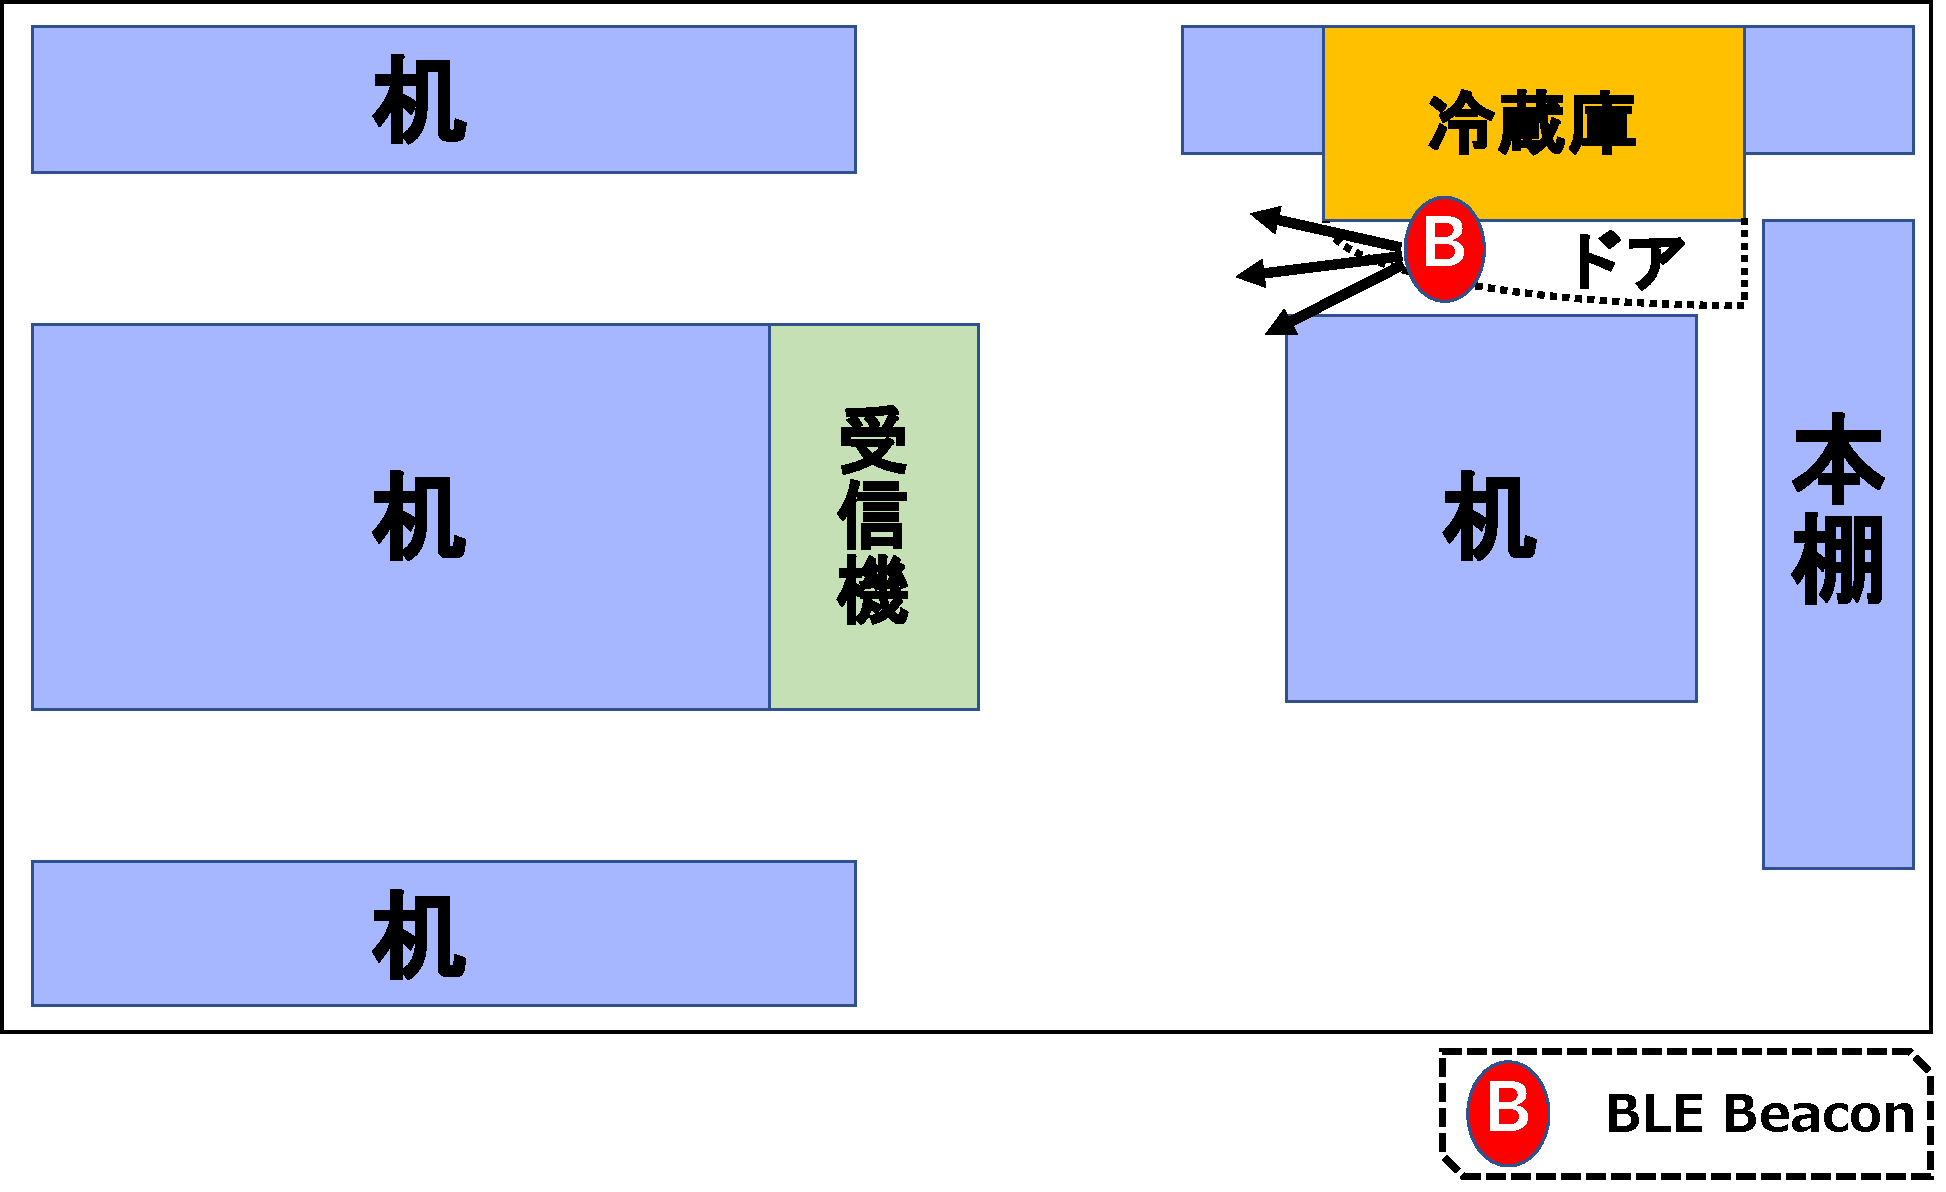
\includegraphics[width=10cm]{images/chapter3/refrigerator_position.pdf}
    \caption{冷蔵庫と受信機の位置関係図}
    \label{refrigerator_position}
\end{figure}


\begin{figure}[tbh]
    \centering
    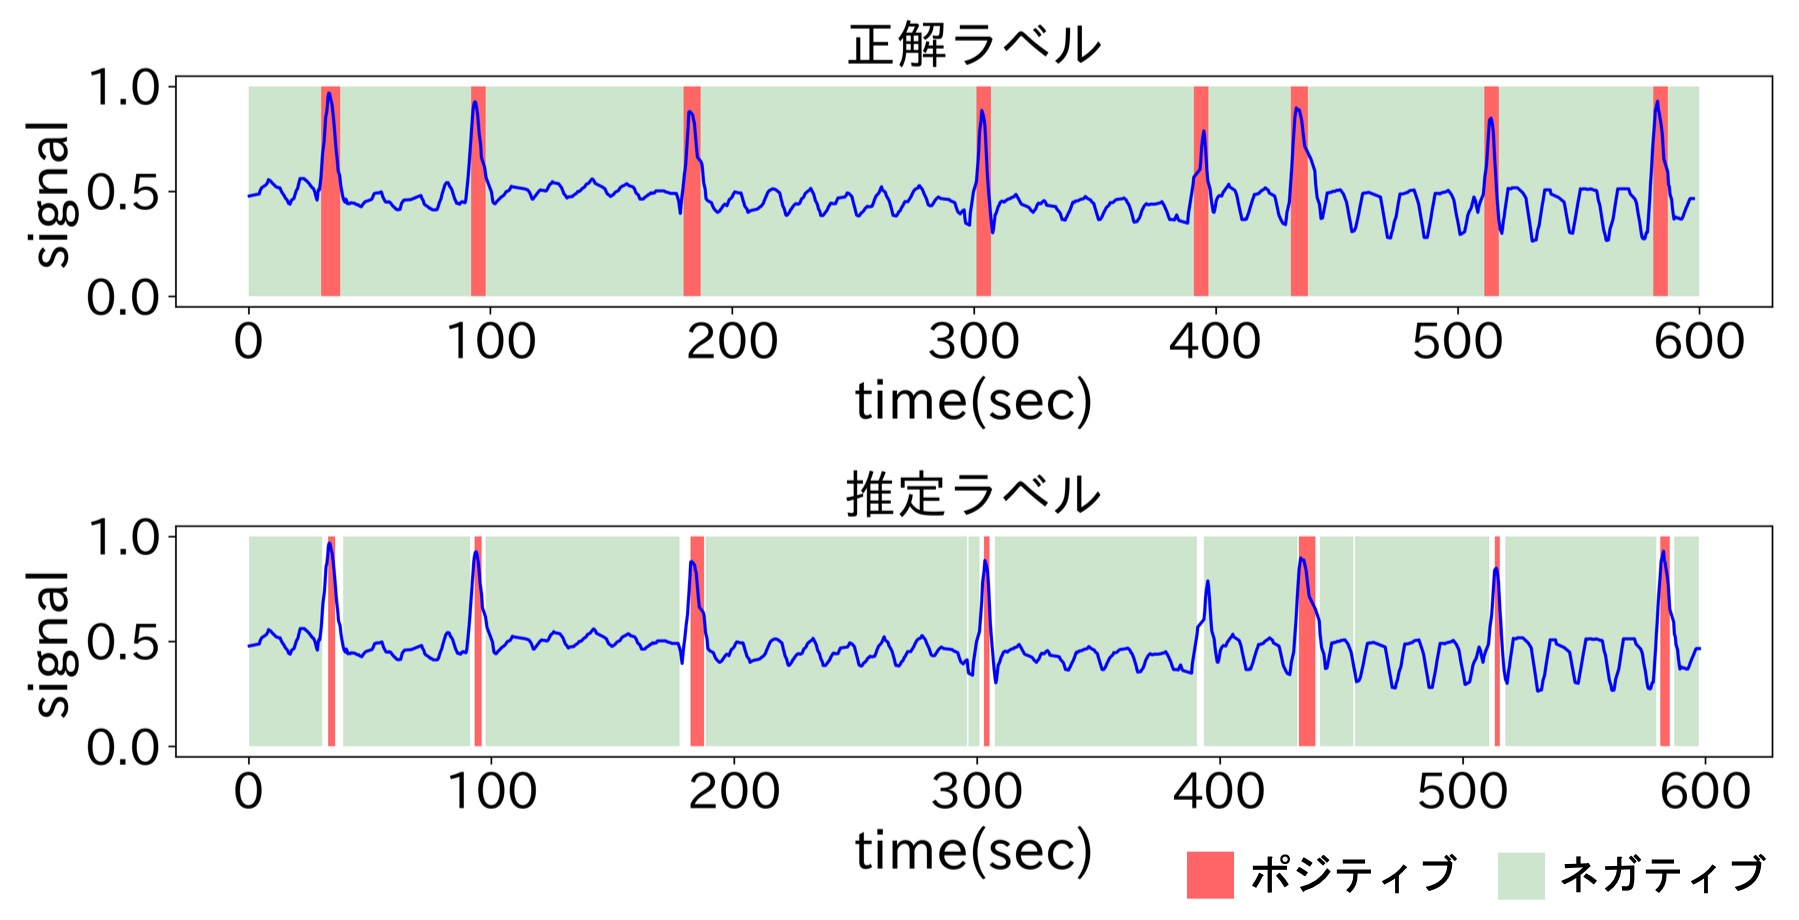
\includegraphics[width=14cm]{images/chapter3/refrigerator_graph.jpg}
    \caption{冷蔵庫の状態推定結果グラフ}
    \label{refrigerator_graph}
\end{figure}


\begin{table}[tbh]
    \begin{center}
        \caption{冷蔵庫の開閉における状態推定精度}
        \label{refrigerator_fig}
        \begin{tabular}{|c|c|c|c|} \hline
        試行回数 & 正答率 & 正解数 & 不正解数 \\ \hline
        1 & 94.1\% & 16 & 1 \\ \hline
        2 & 100\% & 17 & 0 \\ \hline
        3 & 100\% & 17 & 0 \\ \hline \hline
        回数でみた累計正解率 & \multicolumn{3}{c|}{98.0\%} \\ \hline \hline
        推定ラベルの正解割合 & \multicolumn{3}{c|}{99.2\%} \\ \hline
        \end{tabular}
    \end{center}
\end{table}


\subsection{金庫の開閉における推定精度の測定}
図\ref{safe},図\ref{kinko_position}のようにBLEビーコンを設置した金庫と受信機を設置して評価実験を行った.
金庫は図\ref{kinko_position}内に示したの3つの場所でそれぞれ蓋の開閉を行い,推定中にモノの移動が行われても状態推定が可能かを確かめた.
このとき,金庫を開けている時間は約20秒程度であり,閉めた状態はランダムに30秒から2分程度継続させた.
また,安定センシング区間を判定する閾値はそれぞれ,値の閾値を±0.23,時間の閾値を4.5秒に設定した.
推定結果を図\ref{kinko_graph}に,正解率の一覧を表\ref{kinko_fig}に示す.
図\ref{kinko_graph}の白色の範囲は安定センシング区間ではない状態を,緑色の範囲はネガティブな状態(蓋が閉まっている状態)を,赤色の範囲はポジティブな状態(蓋が開いている状態)を示しており,図中の番号は図\ref{kinko_position}内の番号と対応している.

同様の実験を3回行った結果,試行回数をもとにした状態推定精度は100\%,推定ラベルのうち正しく推定できた時間をもとにした状態推定精度は93.8\%であった.

\begin{figure}[tbh]
    \centering
    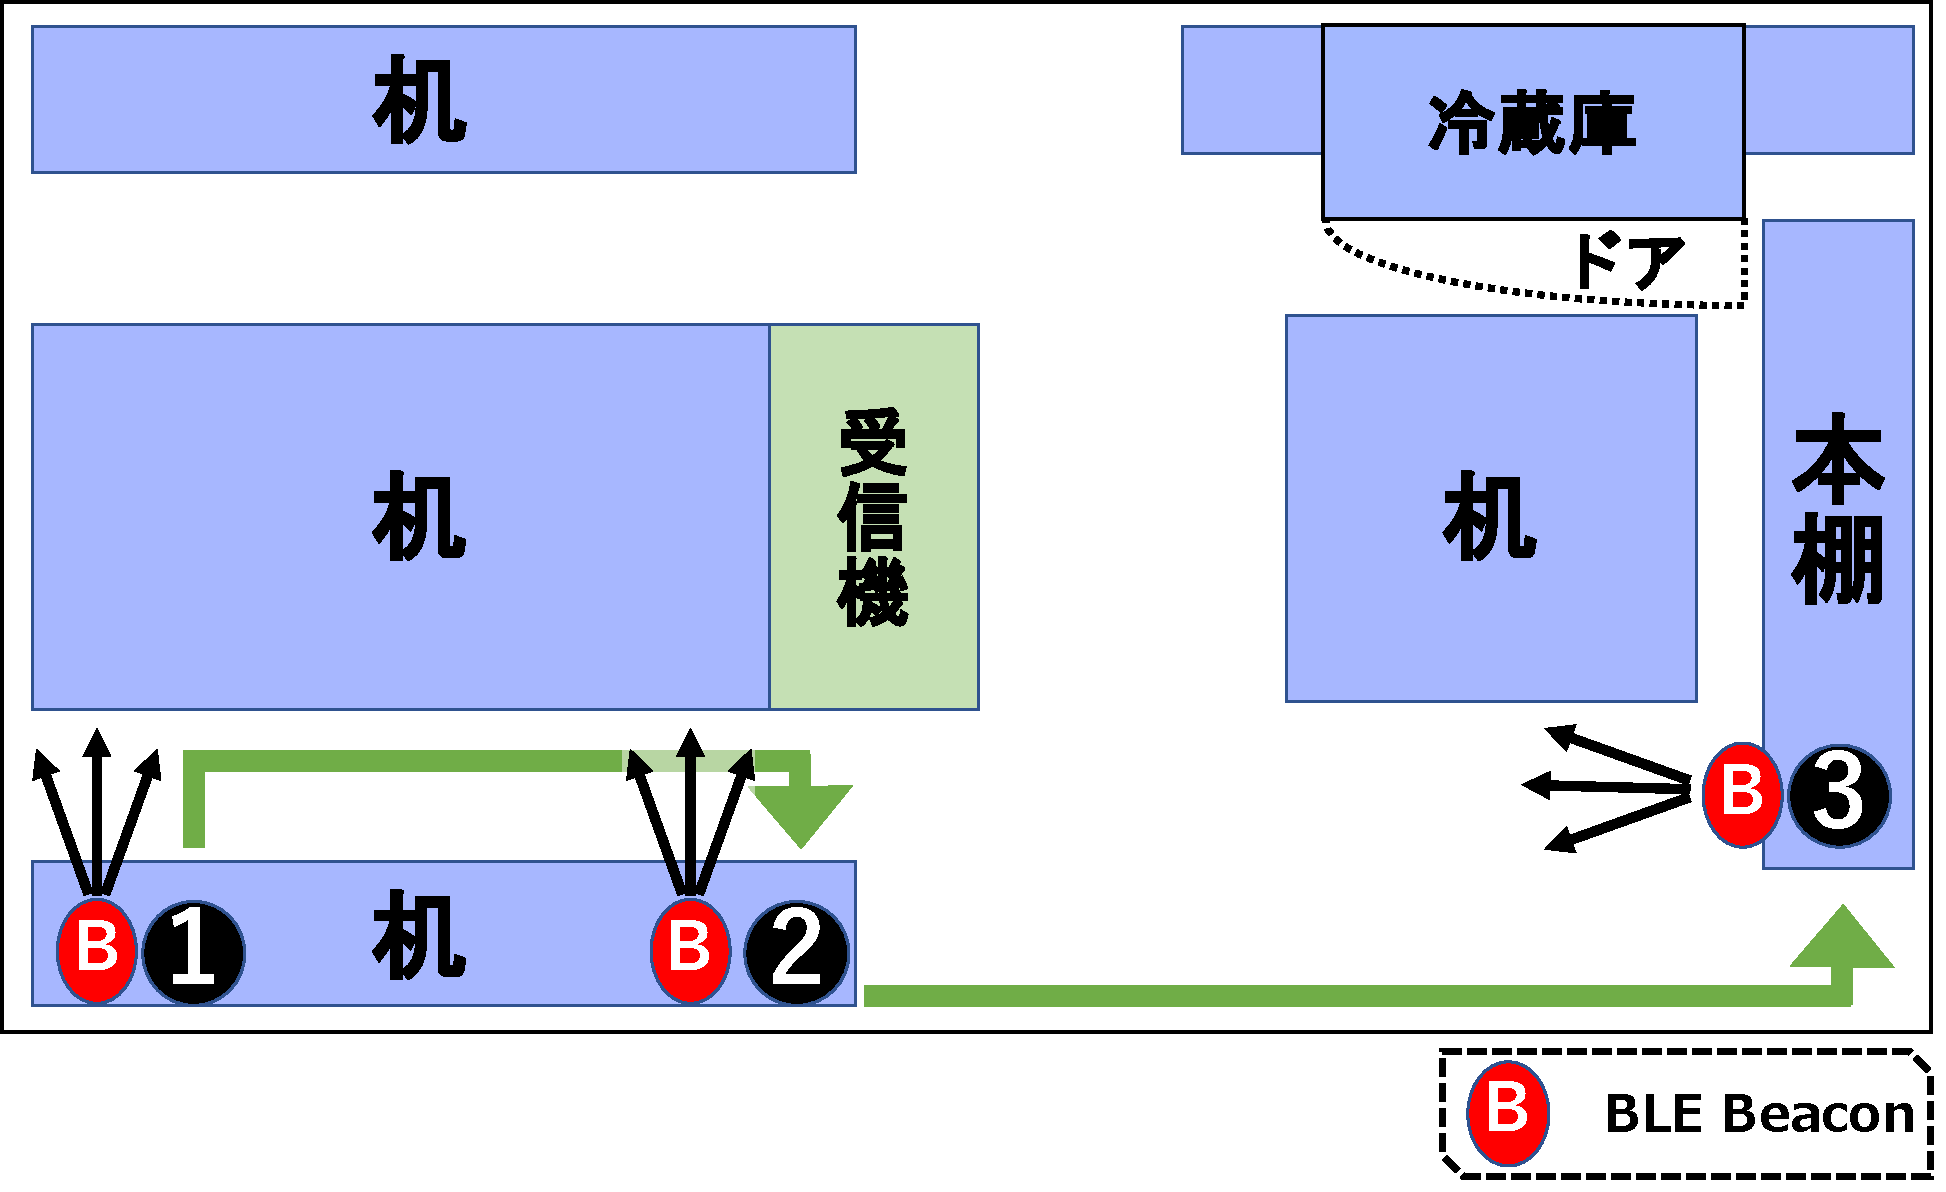
\includegraphics[width=10cm]{images/chapter3/kinko_position_fig.pdf}
    \caption{金庫と受信機の位置関係図}
    \label{kinko_position}
\end{figure}

\begin{figure}[tbh]
    \centering
    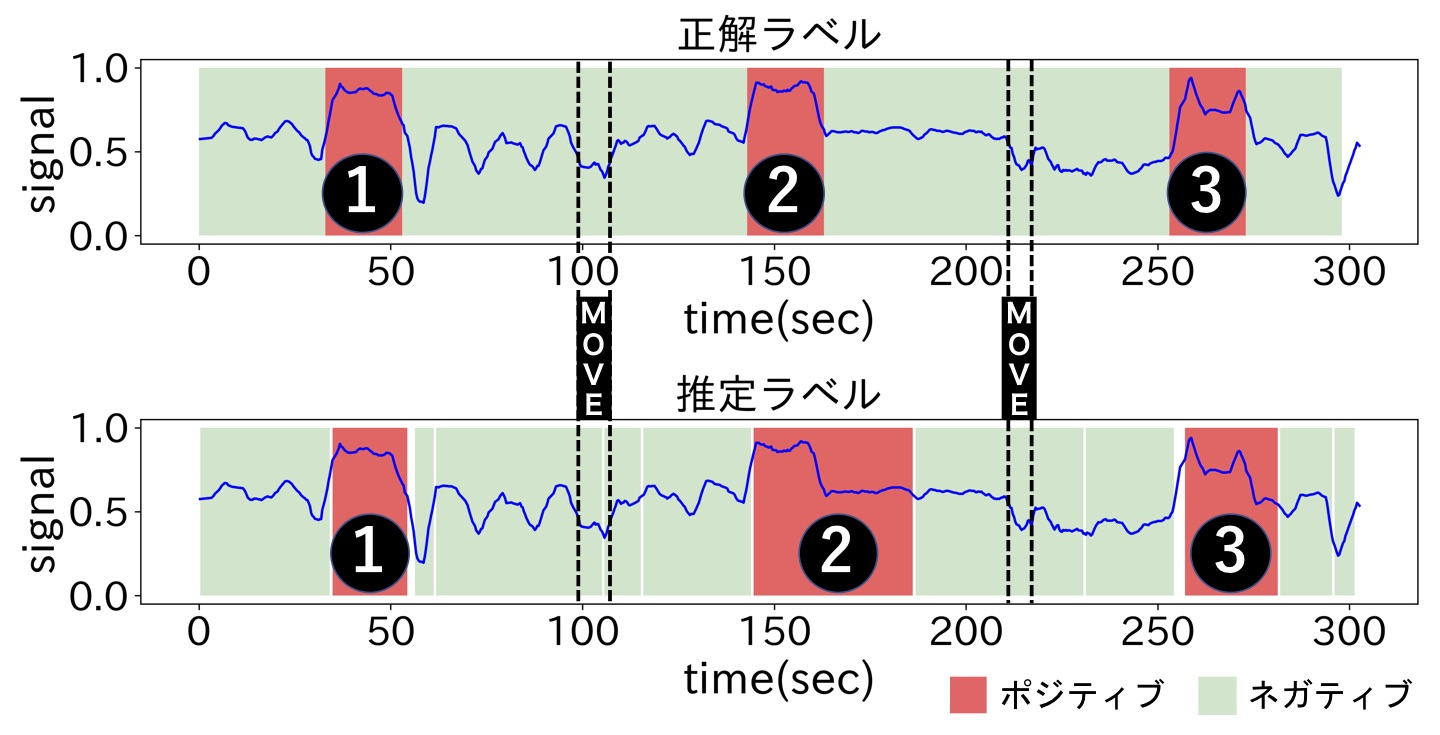
\includegraphics[width=14cm]{images/chapter3/kinko_graph.jpg}
    \caption{金庫の状態推定結果グラフ}
    \label{kinko_graph}
\end{figure}

\begin{table}[tbh]
    \begin{center}
        \caption{金庫の開閉における状態推定精度}
        \label{kinko_fig}
        \begin{tabular}{|c|c|c|c|} \hline
        試行回数 & 正答率 & 正解数 & 不正解数 \\ \hline
        1 & 100\% & 7 & 0 \\ \hline
        2 & 100\% & 7 & 0 \\ \hline
        3 & 100\% & 7 & 0 \\ \hline \hline
        回数でみた累計正解率 & \multicolumn{3}{c|}{100\%} \\ \hline \hline
        推定ラベルの正解割合 & \multicolumn{3}{c|}{93.8\%} \\ \hline
        \end{tabular}
    \end{center}
\end{table}


\subsection{座椅子の着座における推定精度の測定}
図\ref{chair},図\ref{zaisu_position}のようにBLEビーコンを設置した座椅子と受信機を設置して評価実験を行った.
動作の流れとして,1の位置で着座を行った後,2の場所に座椅子を移動させて再度着座を行った.
座椅子に座っている時間として30秒から1分30秒程度を,座っていない時間として30秒から2分程度を設定した.
また,安定センシング区間を判定のための閾値はそれぞれ,値の閾値は±0.235,時間の閾値は5秒に設定した.
推定結果を図\ref{chair_graph}に,正解率の一覧を表\ref{chair_fig}に示す.
図\ref{chair_graph}の白色の範囲は安定センシング区間ではない状態を,緑色の範囲はネガティブな状態(人が座っている状態)を,赤色の範囲はポジティブな状態(人が座っていない状態)を示しており,図中の番号は図\ref{zaisu_position}内の番号と対応している.

同様の実験を3回行った結果,試行回数をもとにした状態推定精度は100\%,推定ラベルのうち正しく推定できた時間をもとにした状態推定精度は98.9\%であった.


\begin{figure}[tbh]
    \centering
    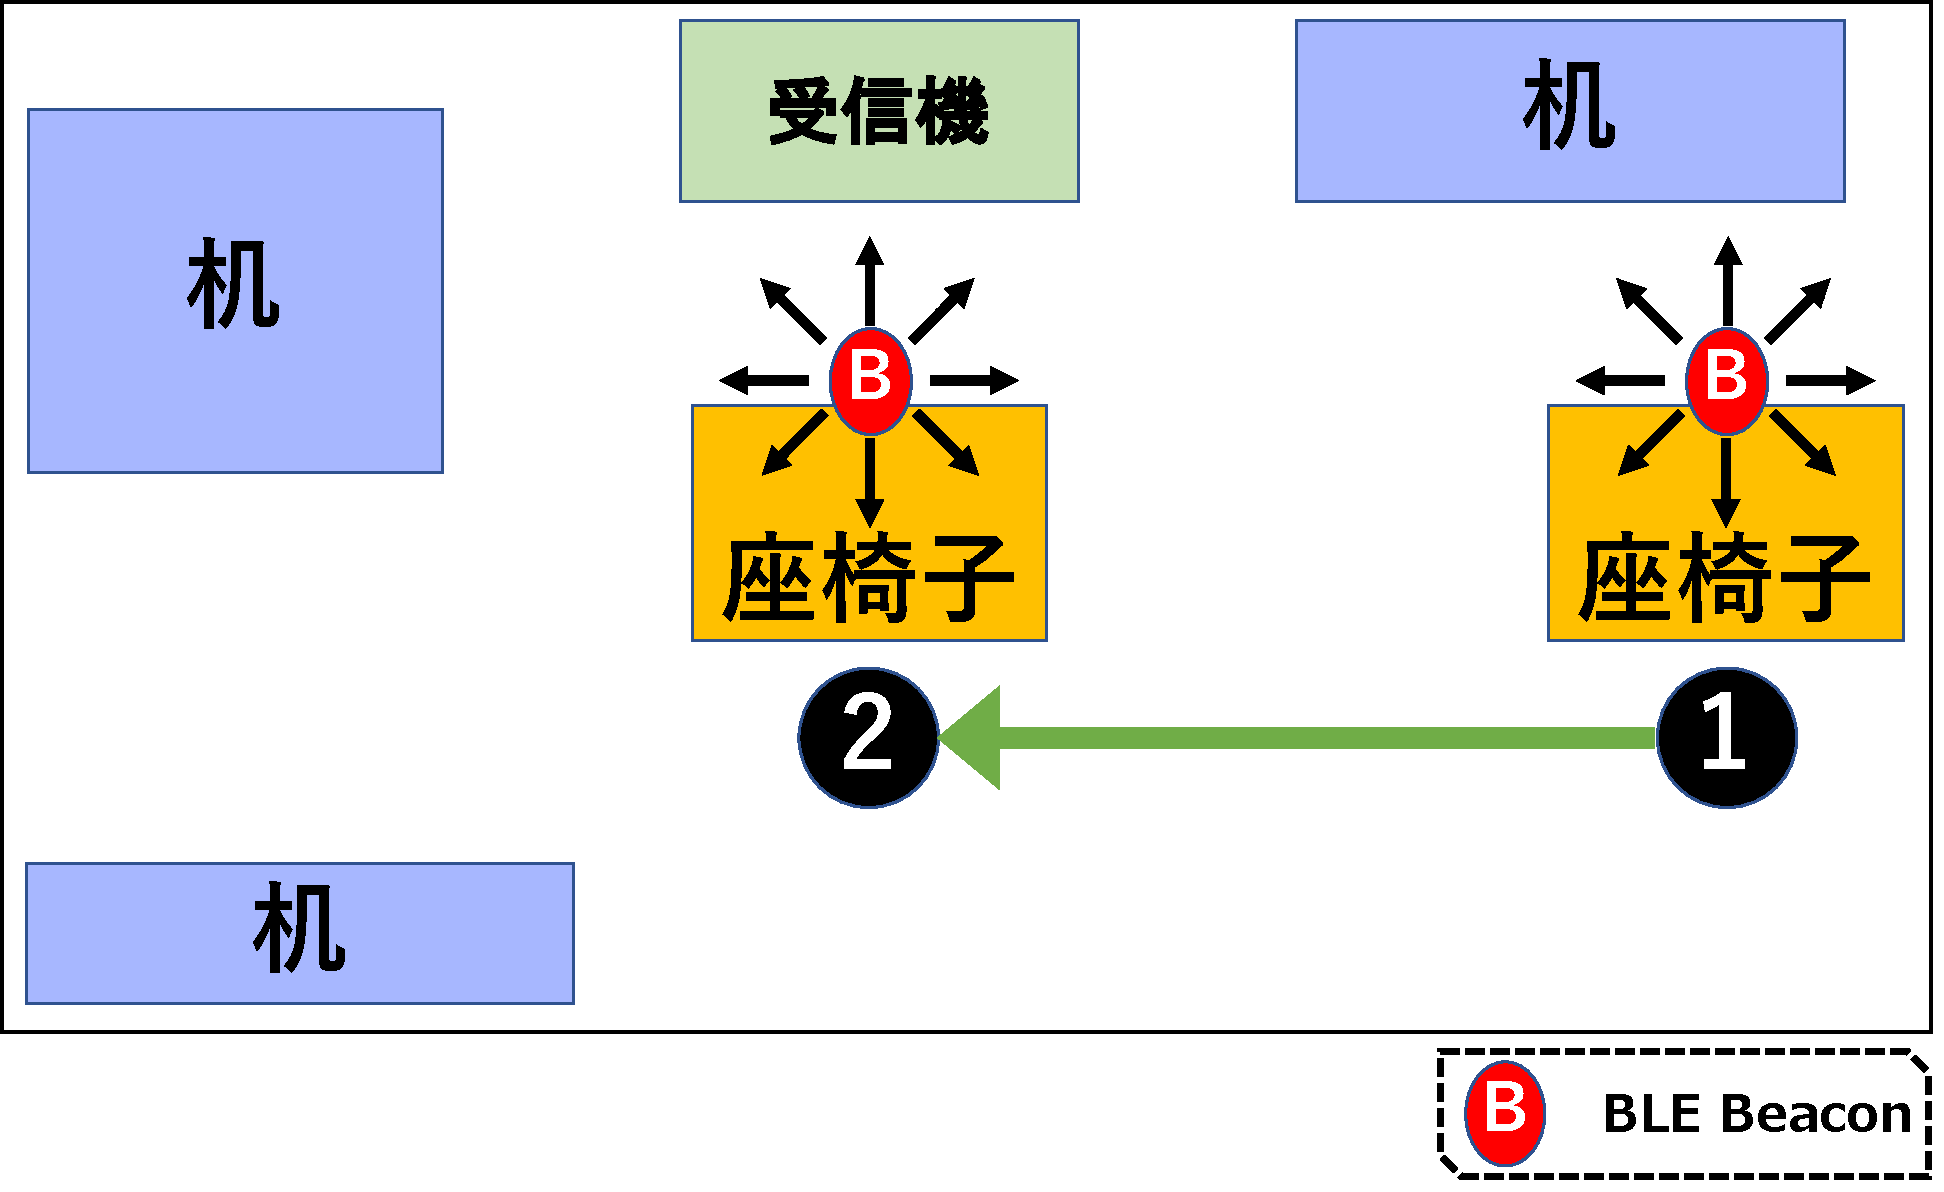
\includegraphics[width=10cm]{images/chapter3/zaisu_position.pdf}
    \caption{座椅子と受信機の位置関係図}
    \label{zaisu_position}
\end{figure}


\begin{figure}[tbh]
    \centering
    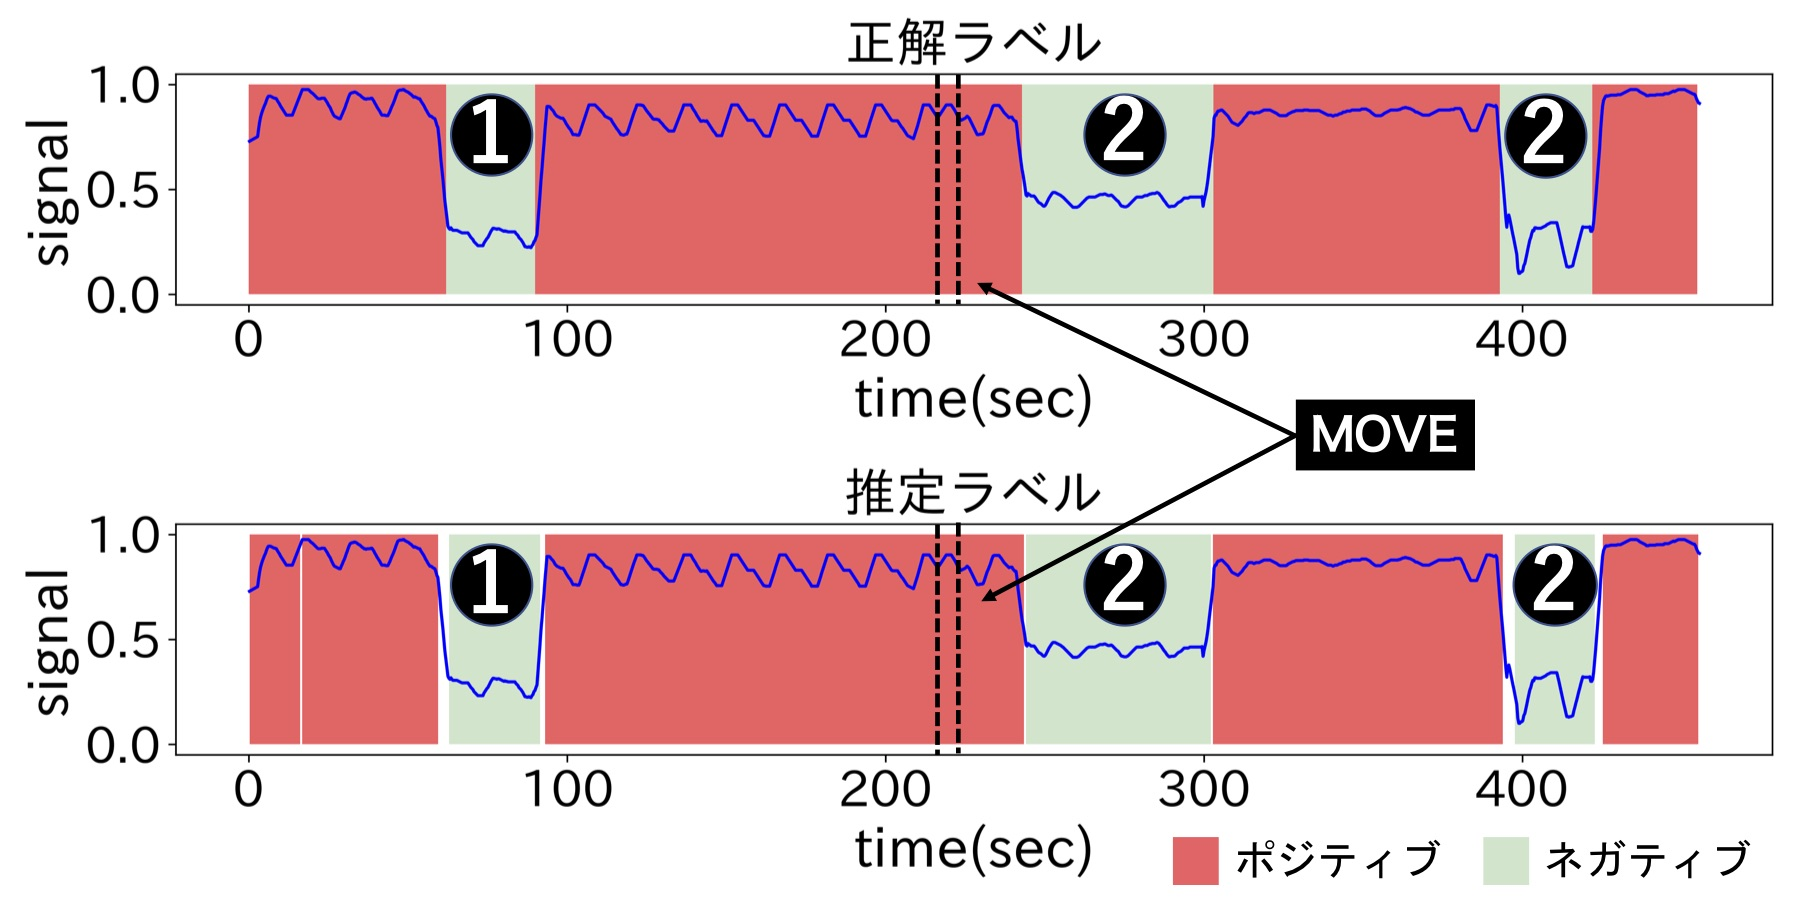
\includegraphics[width=14cm]{images/chapter3/zaisu_graph.jpg}
    \caption{座椅子の状態推定結果グラフ}
    \label{chair_graph}
\end{figure}


\begin{table}[tbh]
    \begin{center}
        \caption{座椅子への着席における状態推定精度}
        \label{chair_fig}
        \begin{tabular}{|c|c|c|c|} \hline
        試行回数 & 正答率 & 正解数 & 不正解数 \\ \hline
        1 & 100\% & 7 & 0 \\ \hline
        2 & 100\% & 7 & 0 \\ \hline
        3 & 100\% & 7 & 0 \\ \hline \hline
        回数でみた累計正解率 & \multicolumn{3}{c|}{100\%} \\ \hline \hline
        推定ラベルの正解割合 & \multicolumn{3}{c|}{98.9\%} \\ \hline

        \end{tabular}
    \end{center}
\end{table}


\section{考察}
評価実験の結果,冷蔵庫の開閉は99.2\%,金庫の開閉は93.8\%,座椅子の着座は98.9\%の精度で推定可能であり,提案手法の有効性を確認できた.
座椅子の状態変化では,受信電波強度が大きく変化したため,安定センシング区間が正解ラベルに近い状態で判定されており,冷蔵庫や金庫より高い推定精度であった.
人体は多く水分を含んでいるため電波を遮りやすく,人が座っていない時と座っている時の電波強度の変化が大きい.
それによりBLEビーコン特有の周期的な電波強度の変化に影響されず,正しく推定ができたと考えられる.

一方で,冷蔵庫と金庫の開閉では安定センシング区間の判定が上手くできていなかったため,誤推定された箇所があった.
これはBLEビーコン特有の周期的な電波強度の変化が安定センシング区間の判定に影響するため,少し大きめの閾値を取った結果,電波強度の変化がこの閾値を超えられなかったと考えられる.
そのため,状態が変化した後であっても前の状態が続いていると判定されてしまい,推定結果にも影響を及ぼした.
従って,推定精度を更に高めるには,安定センシング区間の判定に用いる閾値を見直す必要があるだろう.

%どんなものが出来て出来ないか
本稿の評価実験で扱ったモノの他に,状態変化により電波強度が大きく変化し提案手法が適用できるモノとして,椅子,お店のシャッター,金属製のキャビネットなどいくつかあったが,変化が現れず適用できないモノや状況もあった.
例えば木製のドアや引き出し,ギターケースなどの電波を減衰させにくい材質のモノでは状態変化しても電波強度の変化が少なく状態推定が難しい.
また,提案手法では指向性アダプタを取り付けて電波強度に大きな変化を出すようにしたが,電波が一方向にしか飛ばなくなる.
そのため,指向性アダプタが受信機の方を向いて状態変化が行われないと,電波強度の変化を捉えられないため状態推定を行うのは難しい.

また,本研究では状態がネガティブ・ポジティブの2値であるモノの状態推定を行ってきたが,状態が2値だけでないモノもある.
日常生活空間内にはゴミの累積や服の増減など,状態が推移していくモノもあるためそちらへの対応もする必要もあるだろう.
